\section{UC05 - Visualizzazione dettaglio lampione}\label{uc:05}
\paragraph{Intenzione in contesto} L'attore primario vuole vedere i dettagli di un lampione, di questo vuole conoscerne lo stato.
\paragraph{Attore primario} L'attore primario sono l'utente gestore e manutentore.
\paragraph{Precondizioni}L'attore primario è riconosciuto ed autorizzato dal sistema.
\paragraph{Postcondizioni} L'attore primario visualizza i dettagli e le informazioni su uno specifico lampione.
\paragraph{Scenario principale}
\begin{enumerate}
    \item L'utente richiede di visualizzare i dettagli di uno specifico lampione;
    \item l'utente visualizza i dettagli dello specifico lampione.
\end{enumerate}

\begin{figure}[h]
    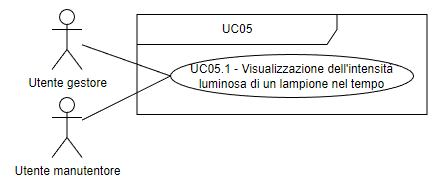
\includegraphics[width=\textwidth]{contenuti/img/casi_uso_grafici-uc05.png}
    \caption{Dettaglio dell'UC05}
    \label{fig:uc05}
\end{figure}

\subsection{UC05.1 Visualizzazione dell'intensità luminosa di un lampione nel tempo}
\paragraph{Intenzione in contesto} L'attore primario desidera visualizzare l'intensità luminosa di un lampione nel tempo.

\paragraph{Attore primario} L'attore primario è l'utente gestore.
\paragraph{Precondizioni}L'attore primario è riconosciuto ed autorizzato dal sistema.
\paragraph{Postcondizioni} L'attore primario visualizza l'intensità luminosa di un lampione nel tempo.

\paragraph{Scenario principale}
\begin{enumerate}
    \item L'utente specifica l'intervallo temporale del quale vuole visualizzare le intensità del lampione;
    \item l'utente visualizza l'intensità del lampione in quell'intervallo temporale.
\end{enumerate}